%You should edit HW.tex, not this file!
\usepackage{mathtools, amsmath, nccmath}
\usepackage{bm}
\usepackage{amsthm}
\usepackage{latexsym}
\usepackage{amssymb}
\usepackage{verbatim}
\usepackage{enumitem,array}
\usepackage{tikz}
\usepackage{color}
\usepackage{bookmark}
\usepackage{geometry}
\geometry{
 a4paper,
 right=15mm,
 left=15mm,
 top = 10mm,
 bottom = 20mm
}
\usepackage{listings}
\usepackage{bussproofs} %for prooftrees
\usepackage{hyperref}
\hypersetup{
	colorlinks=true,
	linkcolor=blue,
	filecolor=magenta,      
	urlcolor=cyan,
}
\usepackage{xepersian}

\definecolor{light-gray}{gray}{0.98}
\definecolor{blue-green}{rgb}{0,0.6,0.5}
\lstset{ 
  backgroundcolor=\color{light-gray},   % choose the background color; you must add \usepackage{color} or \usepackage{xcolor}; should come as last argument
  basicstyle=\footnotesize\color{violet},        % the size of the fonts that are used for the code
  breakatwhitespace=false,         % sets if automatic breaks should only happen at whitespace
  breaklines=true,                 % sets automatic line breaking
  %frame=lines
  captionpos=b,                    % sets the caption-position to bottom
  commentstyle=\itshape\color{blue-green},    % comment style
  %escapeinside={\%*}{*)},          % if you want to add LaTeX within your code
  extendedchars=true,              % lets you use non-ASCII characters; for 8-bits encodings only, does not work with UTF-8
  frame=single,	                   % adds a frame around the code
  keepspaces=true,                 % keeps spaces in text, useful for keeping indentation of code (possibly needs columns=flexible)
  keywordstyle=\bfseries\color{blue},       % keyword style
  %language=Octave,                 % the language of the code
  morekeywords={*,...},            % if you want to add more keywords to the set
  numbers=left,                    % where to put the line-numbers; possible values are (none, left, right)
  numbersep=5pt,                   % how far the line-numbers are from the code
  numberstyle=\tiny\color{gray}, % the style that is used for the line-numbers
  rulecolor=\color{light-gray},         % if not set, the frame-color may be changed on line-breaks within not-black text (e.g. comments (green here))
  showspaces=false,                % show spaces everywhere adding particular underscores; it overrides 'showstringspaces'
  showstringspaces=false,          % underline spaces within strings only
  showtabs=false,                  % show tabs within strings adding particular underscores
  stepnumber=1,                    % the step between two line-numbers. If it's 1, each line will be numbered
  stringstyle=\color{cyan},     % string literal style
  tabsize=2,	                   % sets default tabsize to 2 spaces
  %title=\lstname                   % show the filename of files included with \lstinputlisting; also try caption instead of title
}
%\setlist[enumerate,1]{start=0} %for 0-based enumeration

%\settextfont[
 %BoldFont={HM_XNiloofarBd.ttf}, 
 %ItalicFont={HM_XNiloofarIt.ttf},
 %BoldItalicFont={HM_XNiloofarBdIt.ttf}
 %]{HM_XNiloofar.ttf}
\settextfont{HM XNiloofar}
\ExplSyntaxOn \cs_set_eq:NN \etex_iffontchar:D \tex_iffontchar:D \ExplSyntaxOff
\setdigitfont{HM XNiloofar}
%\setdigitfont{ParsiDigits}
\defpersianfont\outline[Scale=1]{HM XNiloofar Outline}
\setlength{\parindent}{1.5em}
\setlength{\parskip}{0.9em}
\renewcommand{\baselinestretch}{1.5}

%for persian enumeration
\makeatletter
\def\@myharfi#1{\ifcase#1\or آ\or ب\or پ\or ت\or ث\or
ج\or چ\or ح\or خ\or د\or ذ\or ر\or ز\or س\or ش\or ص\or ض\or ع\or غ\or
ف\or ق\or ک\or گ\or ل\or م\or ن\or و\or ه\or ی\else\@ctrerr\fi}
\def\myharfi#1{\expandafter\@myharfi\csname c@#1\endcsname}
\makeatother
\AddEnumerateCounter{\myharfi}{\@myharfi}{}

\newcommand{\lecture}[4]{
%\pagestyle{empty}

	%\begin{center}
	%		\vspace{-1cm}
	%	   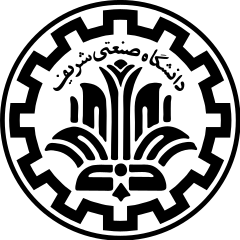
\includegraphics[scale=0.15]{Sharif}%\hfill \\[1em]  
	%\end{center}
	%\vspace{-3em}
\begin{center}

\bf
%\begin{outline} 
{
\LARGE
#1
}
%\end{outline} 
\\
تمرین #2
\end{center}
\vspace*{-1em}
\noindent
نام و نام‌خانوادگی: #3 \hfill شماره دانشجویی: #4
\vspace{-4mm}
\rule{\textwidth}{1pt}
%\ \\
}

% example environment
\newenvironment{example}
{\smallskip \noindent \emph{مثال:}}
{\hfill $\boxtimes$ \smallskip}

\def\Max{\text{بیشینه کن}}
\def\Min{\text{کمینه کن}}
\def\st{\text{\rl{که}}}

\newtheorem{theorem}{قضیه}
\newtheorem{proposition}{گزاره}
\newtheorem*{claim}{ادعا}
\newtheorem*{lemma}{لم}
\newtheorem{numlemma}{لم}
\newtheorem{corollary}{نتیجه}
\newtheorem*{definition}{تعریف} % Use this for non-trivial definitions.
 %%%%%%%%%%%%%%%%%%%%%%%%%%%%%%%%%%%%%%%%%%%%%%%%%%%%%%%%%%%%%%%%%%%%%%%%%%%%

